\documentclass{article}

\usepackage{amsmath}
\usepackage{tikz}

\usetikzlibrary[arrows.meta]

\begin{document}

\section*{Problem 3-3}

\noindent\textbf{\textit{a.}} Not remembering how to asymptotically compare growth rates of functions very well, I'm not very confident in some of these answers. Redefine $>$ into $\Omega$ and redefine $=$ into $\Theta$, for brevity.

First, I placed all functions into rough ``categories'', giving:
\begin{multline}
	\text{Factorial:} ~ (n+1)! ,~ (\log_2 n)! ,~ (n+1)! \\
	\text{Exponential:} ~ 2^{\log_2^* n} ,~ (\sqrt{2})^{\log_2 n} ,~ \left(\frac{3}{2}\right)^n ,~ 2^{2^n} ,~ n \cdot 2^n ,~ 2^{\log_2 n} ,~ e^n ,~ 4^{\log_2 n} ,~ 2^{\sqrt{2 \log_2 n}} ,~ 2^n ,~ 2^{2^{n+1}} \\
	\text{Polynomial:} ~ n^2 ,~ n^3 ,~ n^{\frac{1}{\log_2 n}} ,~ n^{\log_2 \log_2 n} ,~ \left(\log_2 n\right)^{\log_2 n} ,~ \sqrt{\log_2 n} ,~ n ,~ n \log_2 n \\
	\text{Logarithmic:} ~ \log_2 \left(\log^*_2 n\right) ,~ \log^2_2 n ,~ \log_2 (n!) ,~ \ln \ln n ,~ \log^*_2 n ,~ \ln n ,~ \log^*_2 \log_2 n \\
	\text{Constant:} ~ 1 \\
\end{multline}
Second, some work to simplify complex functions:
\begin{eqnarray*}
	4^{\log_2 n} & = & (2^2)^{\log_2 n} \\
	& = & 2^{2 \cdot \log_2 n} \\
	& = & 2^{\log_2 n^2} \\
	& = & n^2 \\
	2^{\log_2 n} & = & n \\
	\sqrt{2}^{\log_2 n} & = & \left(2^{\frac{1}{2}}\right)^{\log_2 n} \\
	& = & 2^{\frac{\log_2 n}{2}} \\
	& = & 2^{\log_2 \sqrt{n}} \\
	& = & \sqrt{n}
\end{eqnarray*}
Third, I sorted the functions as best I could within their categories, giving:
\begin{multline}
	(n+1)! > n! > (\log_2 n)! \\
	2^{2^{n+1}} > 2^{2^n} > e^n > n \cdot 2^n > 2^n > \left(\frac{3}{2}\right)^n > 2^{\sqrt{2 \log_2 n}} > 4^{\log_2 n} > 2^{\log_2 n} > \sqrt{2}^{\log_2 n} \\
	n^{\log_2 \log_2 n} = (\log_2 n)^{\log_2 n} > n^3 > n^2 > n \log_2 n > n > \sqrt{\log_2 n} > n^{\frac{1}{\log_2 n}} \\
	\log_2 (n!) > \log^2_2 n > \ln n > \ln \ln n > \log^*_2 n > \log^*_2 \log_2 n > \log_2 \log^*_2 n \\
	1 \\
\end{multline}
Last, attempting, somewhat blindly, to sort the functions gives:
\begin{multline}
	(n+1)! > n! > 2^{2^{n+1}} > 2^{2^n} > e^n > n \cdot 2^n > \\
	2^n > \left(\frac{3}{2}\right)^n > 2^{\sqrt{2 \log_2 n}} > n^{\log_2 \log_2 n} = \left(\log_2 n\right)^{\log_2 n} > n^3 > \\
	n^2 = 4^{\log_2 n} > n \log_2 n = \log_2 (n!) = \left(\log_2 n\right)! > n = \\
	2^{\log_2 n} > \sqrt{2}^{\log_2 n} > \log^2_2 n > \ln n > \sqrt{\log_2 n} > \ln \ln n > \\
	2^{\log^*_2 n} > \log^*_2 n > \log^*_2 \log_2 n > \log_2 \log^*_2 n > n^{\frac{1}{\log_2 n}} > 1 \\
\end{multline}
...and, though it's probably wrong, I'm going to call that ``good enough'' unless the book cares to instruct me in the finer points of comparing asymptotic growth of slightly-more esoteric equations.

2022-07-28: Comparing my answers with those provided in the instructor's manual, some corrections need to be made, which I'll try to understand and justify below.

First, $2^{2^{n+1}}$ and $2^{2^n}$ are asymptotically greater than $(n+1)!$ and $n!$.  Given equation 3.19:
\begin{eqnarray*}
	\log_2(n!) & = & \Theta(n \log_2(n))
\end{eqnarray*}
From which I'm pretty sure that deriving the following is okay:
\begin{eqnarray*}
	n! & = & \Theta(2^{n \log_2(n)})
\end{eqnarray*}
Comparing $2^{n \log_2(n)}$ and $2^{2^n}$, since $2^n$ is asymptotically greater than $n\log(n)$ it follows that:
\begin{eqnarray*}
	2^{2^n} & = & \Omega(2^{n \log_2 (n)}) \\
	& = & \Omega(n!)
\end{eqnarray*}

Second, $n!$ is asymptotically greater than $e^n$.  Given equation 3.18:
\begin{eqnarray*}
	n! & = & \sqrt{2 \pi n} \left ( \frac{n}{e} \right )^n \left ( 1 + \Theta \left ( \frac{1}{n} \right ) \right ) \\
	 & > & \sqrt{n} \left ( \frac{n}{e} \right )^n ( 1 ) \\
	 & = & n^{n+\frac{1}{2}} e^{-n} \\
	 & > & n^n e^{-n}
\end{eqnarray*}
Multiplying both equations by $e^n$ gives:
\begin{eqnarray*}
	(n^n e^{-n}) e^n = n^n & & e^n e^n = e^{2n} \\
\end{eqnarray*}
Taking the $n$th root of both equations then gives:
\begin{eqnarray*}
	\sqrt[n]{n^n} = n & & \sqrt[n]{e^{2n}} = e^2
\end{eqnarray*}
Since $n$ = $\omega ( e^2 )$, $n! = \omega ( e^n )$.

Third, the equations from $2^{\sqrt{2 \log_2 n}}$ to $\sqrt{2}^{\log_2 n}$ are all kinds of out of order.  Comparing my answers (left) with the provided answers gives: \\
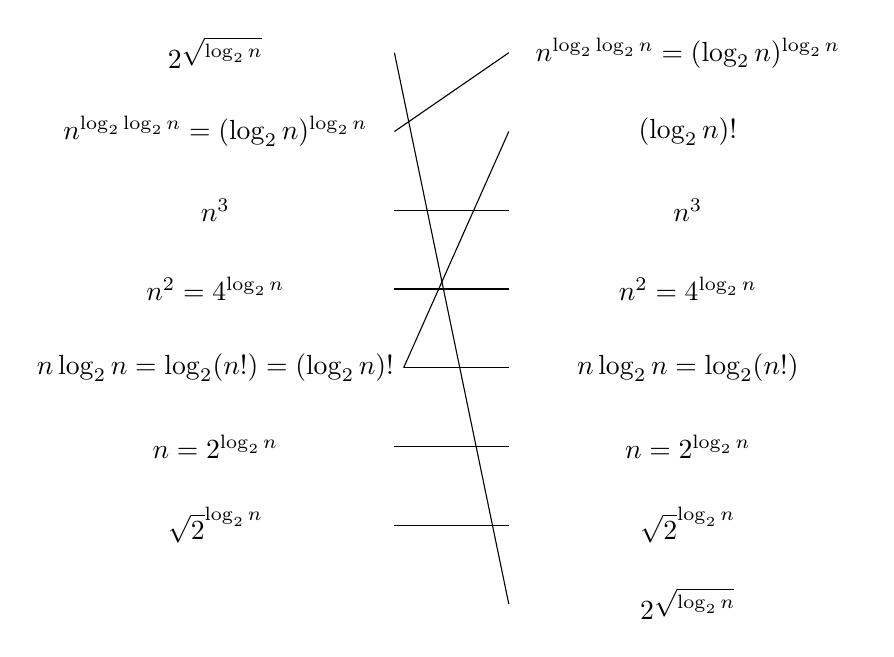
\begin{tikzpicture}
	\newlength{\myleftwidth}
	\settowidth{\myleftwidth}{$n \log_2 n = \log_2 (n!) = (\log_2 n)!$}
	\node (l1) [minimum width=\myleftwidth] at (0,0) {$2^{\sqrt{\log_2 n}}$};
	\node (l2) [minimum width=\myleftwidth] at (0,-1) {$n^{\log_2 \log_2 n} = (\log_2 n)^{\log_2 n}$};
	\node (l3) [minimum width=\myleftwidth] at (0,-2) {$n^3$};
	\node (l4) [minimum width=\myleftwidth] at (0,-3) {$n^2 = 4^{\log_2 n}$};
	\node (l5) [minimum width=\myleftwidth] at (0,-4) {$n \log_2 n = \log_2 (n!) = (\log_2 n)!$};
	\node (l6) [minimum width=\myleftwidth] at (0,-5) {$n = 2^{\log_2 n}$};
	\node (l7) [minimum width=\myleftwidth] at (0,-6) {$\sqrt{2}^{\log_2 n}$};

	\newlength{\myrightwidth}
	\settowidth{\myrightwidth}{$n \log_2 n = \log_2 (n!) = (\log_2 n)!$}
	\node (r1) [minimum width=\myrightwidth] at (6, 0) {$n^{\log_2 \log_2 n} = (\log_2 n)^{\log_2 n}$};
	\node (r2) [minimum width=\myrightwidth] at (6, -1) {$(\log_2 n)!$};
	\node (r3) [minimum width=\myrightwidth] at (6, -2) {$n^3$};
	\node (r4) [minimum width=\myrightwidth] at (6, -3) {$n^2 = 4^{\log_2 n}$};
	\node (r5) [minimum width=\myrightwidth] at (6, -4) {$n\log_2 n = \log_2(n!)$};
	\node (r6) [minimum width=\myrightwidth] at (6, -5) {$n = 2^{\log_2 n}$};
	\node (r7) [minimum width=\myrightwidth] at (6, -6) {$\sqrt{2}^{\log_2 n}$};
	\node (r8) [minimum width=\myrightwidth] at (6, -7) {$2^{\sqrt{\log_2 n}}$};

	\draw (l1.east) -- (r8.west);
	\draw (l2.east) -- (r1.west);
	\draw (l3.east) -- (r3.west);
	\draw (l4.east) -- (r4.west);
	\draw (l5.east) -- (r2.west);
	\draw (l5.east) -- (r5.west);
	\draw (l6.east) -- (r6.west);
	\draw (l7.east) -- (r7.west);
\end{tikzpicture} \\
To convince myself of the correctness of this, I will prove the following based off of the provided justifications:
\begin{enumerate}
	\item $(\log_2 n)! = O(n^{\log_2 \log_2 n})$
	\item $(\log_2 n)! = \Omega(n^3)$
	\item $2^{\sqrt{2 \log_2 n}} = O(\sqrt{2}^{\log_2 n})$
\end{enumerate}
For \#1, begin with Stirling's approximation:
\begin{eqnarray*}
	n! &=& \sqrt{2 \pi n} \left ( \frac{n}{e} \right )^n \left ( 1 + \Theta \left ( \frac{1}{n} \right ) \right ) \\
	(\log_2 n)! &=& \sqrt{2 \pi \log_2 n} \left ( \frac{\log_2 n}{e} \right )^{\log_2 n} \left ( 1 + \Theta \left ( \frac{1}{\log_2 n} \right ) \right )
\end{eqnarray*}
Dropping constants and low-order terms gives:
\begin{eqnarray*}
	(\log_2 n)! &=& \sqrt{\log_2 n} \left ( \frac{\log_2 n}{e} \right )^{\log_2 n} (1) \\
	&=& \sqrt{\log_2 n} \left ( \frac{(\log_2 n)^{\log_2 n}}{e^{\log_2 n}} \right ) \\
	&=& \sqrt{\log_2 n} \left ( \frac{(\log_2 n)^{\log_2 n}}{n^{\log_2 e}} \right ) \\
	&=& \frac{\sqrt{\log_2 n}}{n^{\log_2 e}} ( \log_2 n )^{\log_2 n}
\end{eqnarray*}
Since $\frac{\sqrt{\log_2 n}}{n^{\log_2 e}} \rightarrow 0$ as $n \rightarrow \infty$:
\begin{eqnarray*}
	(\log_2 n)! &=& o(\log_2 n)^{\log_2 n}
\end{eqnarray*}
For \#2, use equation 3.19 for the first equation and then subtitute $\log_2 n$ for $n$ in both equations:
\begin{eqnarray*}
	\log_2 (n)! & = & \Theta (n \log_2 n) \\
	\log_2 (\log_2 n)! & = & \Theta (\log_2 n \log_2 \log_2 n)
\end{eqnarray*}
and:
\begin{eqnarray*}
	\log_2 n^3 & = & 3 \log_2 n
\end{eqnarray*}
Comparing the two gives:
\begin{eqnarray*}
	\log_2 n \log_2 \log_2 n &   & 3 \log_2 n \\
	\log_2 \log_2 n &   & 3 \\
	& = & \omega(3)
\end{eqnarray*}
For \#3, simplify the right side:
\begin{eqnarray*}
	\sqrt{2}^{\log_2 n} & = & 2^{\frac{1}{2} \cdot \log_2 n} \\
	& = & 2^{\log_2 \sqrt{n}} \\
	& = & \sqrt{n} \\
\end{eqnarray*}
then take the base 2 logarithm of both equations:
\begin{eqnarray*}
	\log_2 \sqrt{n} & = & \frac{1}{2} \log_2 n
\end{eqnarray*}
and:
\begin{eqnarray*}
	\log_2 2^{\sqrt{2 \log_2 n}} & = & \sqrt{2 \log_2 n} \\
	& = & \sqrt{2} \log_2^{\frac{1}{2}} n
\end{eqnarray*}
Since $\log_2 n = \omega (\log_2^{\frac{1}{2}} n)$, $\log_2^{\frac{1}{2}} n = o(\log_2n)$ and thus $2^{\sqrt{2 \log_n}} = O \sqrt{2}^{\log_2 n}$.

Fourth, though it wasn't justified in the provided answers, I wanted to see if I could figure out why $\left ( \frac{3}{2} \right )^n = \Omega(n^{\log_2 \log_2 n})$.  Taking the base 2 logarithm of both sides gives:
\begin{eqnarray*}
	\log_2 (3/2)^n = \log_2 (3^n 2^{-n})	&|& \log_2 ( n^{\log_2 \log_2 n} ) = \log_2 \log_2 n \log_2 n \\
	= \log_2 3^n + \log_2 2^{-n} 		&|& < \log_2 n \log_2 n \\
	= n\log_2 3 - n				&|& = \log_2^2 n \\
	\approx 0.585n				&|&
\end{eqnarray*}
Taking the square root of both sides then gives:
\begin{eqnarray*}
	\sqrt{0.585} \sqrt{n} 			&|& \sqrt{\log_2^2 n} = \log_2 n
\end{eqnarray*}
Since $\sqrt{n} = \omega (\log_2 n)$, $\left ( \frac{3}{2} \right )^n = \Omega (n^{\log_2 \log_2 n})$.

Fifth, rather than $\log_2^* n > \log_2^* \log_2 n$, $\log_2^* n = \log_2^* \log_2 n$ because applying the logarithm before applying the iterated logarithm function is merely a pre-application which lowers the number of iterated logarithm function iterations by one but does not lower the overall number of iterations (unless $n < 4$).

Sixth, as per identity 4, since $n^{\frac{1}{\log_2 n}} = 2$, rather than $n^{\frac{1}{\log_2 n}} = \omega(1)$, $n^{\frac{1}{\log_2 n}} = \Theta (1)$.
\end{document}
